
\section{Introduzione} % Sections are added in order to organize your presentation into discrete blocks, all sections and subsections are automatically output to the table of contents as an overview of the talk but NOT output in the presentation as separate slides

%------------------------------------------------

\begin{frame}
\frametitle{Transformer}
\textbf{Self-attention-based architectures}, in particular Transformers, have become the model of choice in natural language processing.
\vspace{0.5cm}

The dominant approach is to pre-train on a \textbf{large text corpus and then fine-tune on a smaller task-specific dataset}.

\end{frame}

\begin{frame}
\frametitle{What computer vision?}
In computer vision, however, \textbf{convolutional architectures remain dominant}.
Multiple works try combining \textbf{CNN-like architectures with self-attention}, while theoretically efficient, have not yet been scaled effectively on modern hardware accelerators due to the use of specialized attention patterns. 
\end{frame}

\begin{frame}
\frametitle{What computer vision?}
With Vision transformer the end goal is to \textbf{apply a standard Transformer directly to images}, with the fewest possible modifications
\begin{center}
    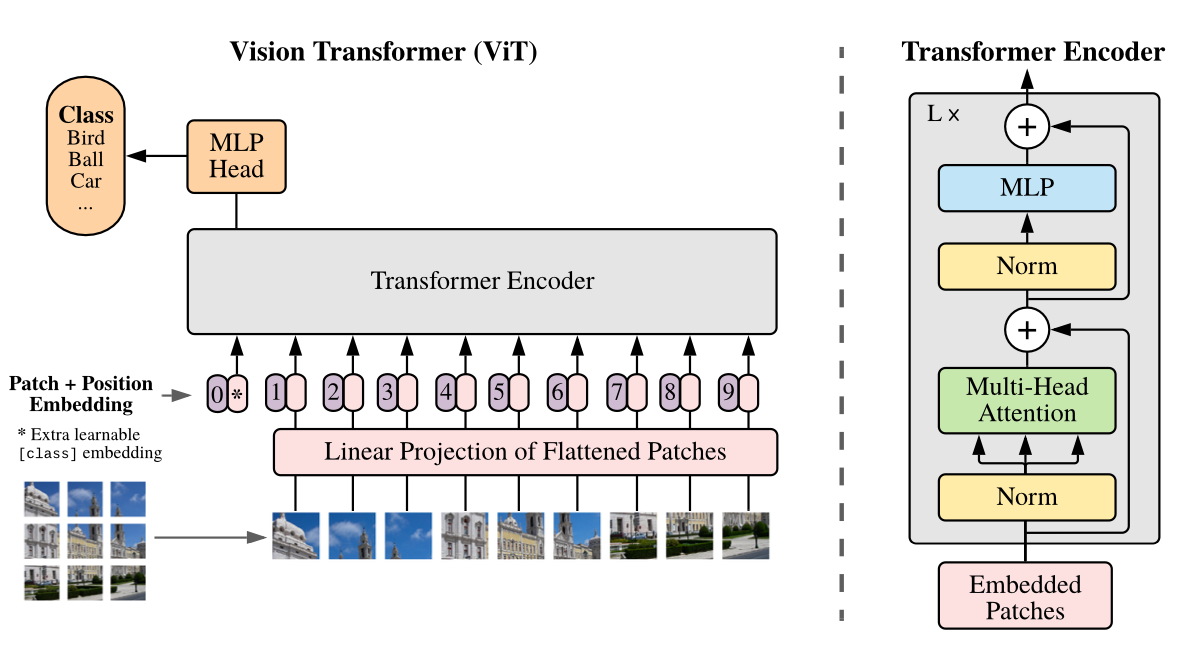
\includegraphics[width=0.8\textwidth]{img/1-section/Vision transformer.png} 
\end{center}

\end{frame}